%!TEX ROOT=sample-thesis.tex
%!TEX PROGRAM=xelatex

\chapter{Methodology}

This chapter presents the detailed descriptions and justifications of the methodology used to achieve the research objectives. This chapter explains the methods used in this study into three major sections: problem characterization and abstraction, design development and implementation, and design evaluation and validation. Detailed characterization and abstraction of domain problems helps in deriving design requirements in generating appropriate visualization solutions. A literature review and a case study were carried out to elicit a problem abstraction based on data, users, and tasks. A visual analytics design was designed based on the identified requirements from the characterization and abstraction. Design experience on constructing the design including design consideration and rationales are also discussed. Finally, this chapter then introduces the user study methodology to evaluate and validate the design. Detailed descriptions of the user study methodology including think-aloud observation and expert validation interview are elaborated.
\\[\baselineskip]\indent
This chapter is organized as follows. Section 3.1 presents the domain problem characterization and abstraction for MOOC analytics. Detailed descriptions including the fundamentals of problem characterizations, user study methodology, and characterizations results are presented. In Section 3.2, detailed characteristics of domain and user requirements including data descriptions, tasks, and target user are described. Subsequently, design experience on the proposed design including design consideration and rationales to facilitate each domain problem are discussed. Section 3.3 then introduces the user case study methods used for evaluating and validating the proposed design. Detailed descriptions and justifications of protocols and instruments for think-aloud observation and expert validation are presented. Lastly, the chapter is concluded in Section 3.4.

\section{Problem Characterization and Abstraction for MOOC Analytics}
This section firstly introduces the concept and example studies of problem characterization and abstraction. Next, discussions on related literature on visual analytics and visualization for MOOC are presented. Subsequently, detailed descriptions of case study method to extract domain problem characterization and abstraction are described. This section then presents and discuss the findings from the problem characterization to be design references in facilitating MOOC learner support monitoring.

\subsection{Problem Characterization and Abstraction}
There are limited existing visualization research focusing on problem-oriented visualization despite its importance in visual analytics design and implementation (Lam et al., 2012). To encourage problem-oriented approach in visualization, the design study methodology is introduced \parencite{Sedlmair2012}. This methodology leverages detailed problem characterization and abstraction in designing visual analytics solution. Notable examples of problem characterization and abstraction in design studies across domains are discussed as follows.
\\[\baselineskip]\indent
\textcite{Wagner2014} investigated the design requirements of visual analytics for behavior-based malware pattern analysis \parencite{Wagner2014}. They characterized the design requirements based on problem characterization and abstraction using literature, user focus groups, and expert interviews.
\\[\baselineskip]\indent
\textcite{Riveiro2017} then conducted a design study on facilitating visual analysis in anomaly detection on multidimensional transport traffic data \parencite{Riveiro2017}. Their design framework was implemented and demonstrated on European real transport traffic data. Furthermore, expert analysts from industrial organization were interviewed for evaluating the usability of the proposed design framework.

\begin{figure}[hbt!]
\centering
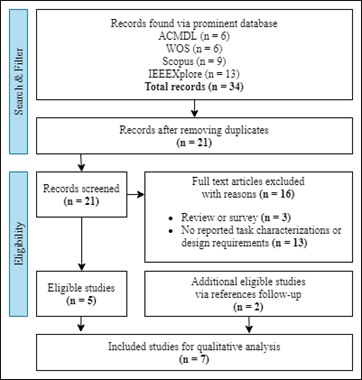
\includegraphics[scale=1]{Fig3.2}
\caption{Literature review workflow for problem characterizations}
\end{figure}

\bigskip

\begin{table}[hbt!]
\caption{Inclusion and exclusion criteria for literature selection for review}
\centering
\begin{tabular}{ p{1.5cm} p{5cm} p{6.5cm} }
\hline
No.	& Criteria & Justification \\ \hline
1 	& The study must be an original research paper instead of a review or survey paper. & Review and survey papers do not always contain a sufficient description of design studies or detailed problem characterizations. \\
\hline
\end{tabular}
\end{table}

\subsubsection{Expert Interview}
To help characterize domain analysis tasks and user requirements, several MOOC experts were recruited from the education field in Malaysia. An interview protocol was designed for the semi-structured interview sessions as follows.
\\ \\
a.	Identify \\
\indent $OI_1$ \indent Total number of learners in the course. \\
\indent $OI_2$ \indent Percentage of learners with age between 35 and 55 years old. \\
\indent $OI_3$ \indent Number of categories for learners’ academic background. \\
\indent $OI_4$ \indent List 3 learners who completed the course with distinction.
\\ \\
b.	Find extremum \\
\indent $OE_1$ \indent Month with highest number of registrations, and then withdrawals. \\
\indent $OE_2$ \indent Largest group of learners by their academic background. \\
\indent $OE_3$ \indent Smallest group of learners by their final grade.
\\ \\

\begin{table}[hbt!]
\caption{Justification of pre-defined tasks during analysis scenario on Overview view}
\centering
\begin{tabular}{ |c|c|c|c| }
\hline
Hey & How's it & Going?\\ \hline
Fine! & Just great. & See ya!\\
Fine! & Just great. & See ya!\\
\hline
\end{tabular}

\source{The Source.}
\end{table}

Time for some maths.
\begin{equation}
\left[M\frac{\partial }{\partial M}+\beta(g)\frac{\partial }{\partial g}+n\gamma\right] G^{(n)}(x_1,x_2,\ldots,x_n;M,g)=0,
\end{equation}
